%\section{Project Logic}
\chapter{Project Logic}
\label{chap:logic}
%\pagenumbering{arabic}

In this work we started considering the features and problems recognizable as a Farm parallel pattern.
Then the study moved to consider how a GPU works, its main architectural characteristics and facing its data parallel nature.
Next we had to think how to "merge" two such different behaviors, in order to reach reasonable performances\footnote{About expected performances see \hyperref[sect:overallLogic]{Section 3.3} and \hyperref[sect:tunings]{Section 3.4} for more clarifications.}, i.e. almost competitive with a classic data parallel problem.
Finally, once the main idea behind the development was clear, we had to make some tunings.
All of these steps will be shown in detail in next sections.

\section{Stream Parallelism: Farm pattern}

	Stream parallel patterns describe problems exploiting parallelism among computations relative to different independent data items, appearing on the program input stream at different times.
	Each independent computation ends with the delivery of one single item on the program output stream.\\
	We focused on \textbf{Farm parallel pattern}, modeling embarrassingly parallel stream parallelism.\\
	The only functional parameter of a farm is the function \(f\) needed to compute the single task\cite{spm}.
	Given a stream of input tasks 
	\begin{center}
		\(x_m , . . . , x_1\)\\
	\end{center}
	the farm with function \(f\) computes the output stream as
	\begin{center}
		\(f ( x_m ), . . . , f ( x_1 )\)
	\end{center}
	Its parallel semantics ensures it will process the single task in a time close to the time needed to compute \(f\) sequentially. The time between the delivery of two different task results, instead, can be made close to the time spent to compute f sequentially divided by the number of parallel agents used to execute the farm, i.e. its parallelism degree\cite{spm,parpattbench}.\\


The correspondent task farm skeleton, with a parallelism degree parameter, may therefore be defined with
the high order function description:\\
\texttt{let rec farm f =}
	
	\texttt{function}
	
	\texttt{EmptyStream -> EmptyStream}
	
	\texttt{| Stream(x,y) -> Stream((f x),(farm f y));;}\\\\
	%
whose type is

\( farm :: (\alpha \rightarrow \beta) \rightarrow \alpha \  stream \rightarrow \beta \ stream \)\\\\
%
%
\textit{The parallel semantics, associated to the higher order functions, states that the computation of any item appearing on the input stream may be performed in parallel}, according to the number of available workers\cite{spm}.\\

In the farm case, according to the parallel semantics a number of parallel agents, computing function \(f\) onto input data items, equal to the number of items appearing onto the input stream could be used. This is not realistic, however, for two different reasons:

\begin{enumerate}
	\item items in the stream do not exist all at the same time, since a stream is not a vector.
	Items of the stream do appear at different times. Actually, when we talk of consecutive items \(x_{i}\) and \(x_{i+1}\) of the stream we refer to items appearing onto the stream at times \(t_{i}\) and \(t_{i+1}\) with \(t_{i} < t_{i+1}\). As a consequence, it makes no sense to have a distinct parallel agent for all the items of the input stream, as at any given time only a fraction of the input stream will be available.
	
	\item if we use an agent to compute item \(x_{k}\), presumably the computation will end at some
	time \(t_{k}\). If item \(x_{j}\) appears onto the input stream at a time \(t_{j} > t_{k}\) this same agent can be used to compute item \(x_{j}\) rather than picking up a new agent. \\
\end{enumerate}
This is why the parallelism degree of a task farm is a critical parameter: a small parallelism degree doesn't exploit all the parallelism available (thus limiting the speedup), while a large parallelism degree may lead to inefficiencies as part of the parallel agents will be probably idle most of time\cite{spm}.\\


\subsection{Farm performance model}
\label{subs:farmperfmodel}
	It's important to consider which kind of performance indicators are useful. When dealing with performances of parallel applications, we are in general interested in two distinct kind of measures:
	\begin{itemize}
		\item those measuring the absolute (wall clock) time spent in the execution of a given (part of) parallel application. Here we can include measures such as
		\begin{enumerate}
			\item \textbf{Latency} (\(L\)). The time spent between the moment a given activity receives input data and	the moment the same activity delivers the output data corresponding to the input.
			\item \textbf{Completion time} (\(T_c\)). The overall latency of an application computed on a given input data set, that is the time spent from application start to application completion.
		\end{enumerate}
		\item those measuring the throughput of the application, that is the rate achieved in the delivering of the results. Here In this case we can include measures such as
		\begin{enumerate}
			\item \textbf{Service time} (\(T_s\)). The time intercurring between the delivery of two successive output items (or alternatively, the time between the acceptance of two consecutive input items), and
			\item \textbf{Bandwidth} (\(B\)). The inverse of the service time.
		\end{enumerate}
	\end{itemize}
	These are the basic performance measures of interest in parallel/distributed computing.
	Applications with a very small service time (a high bandwidth) have a good throughput but not necessarily small latencies\cite{spm}.\\
	As an example, if we are interested in completing a computation within a deadline, we will be interested in the application completion time rather than in its service time.\\
	Each performance measure has an associated “semantics”:
	\begin{itemize}
		\item	\(L, T_c\) the latency and the completion time represent “wall clock time” spent in computing a given parallel activity. We are interested in minimizing latency when we want to complete a computation as soon as possible;
		\item \(T_s, B\) service time represents (average) intervals of time incurring between the delivery (or acceptance) of two consecutive results (or tasks). We are interested in minimizing service time when we want to have results output as frequently as possible, but we don't care of latency in the computation of a single result. As bandwidth is defined as the inverse of the service time, we are interested in bandwidth maximization in the very same cases\cite{spm}.
	\end{itemize}

	Given those measures of interest, we can describe an \textit{approximate performance model} for Farm parallel pattern.\\
	First we start considering the service time strictly for workers activity
	\begin{equation}
		T_s = \frac{T_w}{n_w}
	\end{equation}
	So in task farm, the service time is given by the service time of the workers (\(T_w\)) in the farm, divided by the number of workers (\(n_w\)), as hopefully \(n_w\) results will be output by the workers every \(T_w\) units of time\cite{spm}.
	
	We can add to this model the times spent by emitter and collector, but this will depend strictly on how the Farm is implemented. For example, suppose we have an emitter/collector single process, it gathers input tasks from the input stream and schedules these tasks for execution on one of the available workers. Workers, in turn, receive tasks and once workers compute tasks, they send back to the emitter/collector process the results\footnote{The emitter/collector process \textendash concurrently to its task scheduling	activity\textendash  collects results, possibly re-order them to respect the input task order in the output sequence too.}.
	This template is often referred to as \textit{master-worker pattern}.\\
	% although–in our perspective–this is actually a template suitable to implement both the task farm and map/data parallel skeletons.}.

	The three activities \textendash task scheduling, task computation and results gathering and dispatching \textendash happen to be executed in pipeline\footnote{A performance model of the pipeline service time states that its service time is the maximum of the service times of the pipeline stages, as it is known that the slowest pipeline stage, sooner or later, will behave as the	computation bottleneck.}. Therefore the service time of the master worker is approximated by the maximum of the service times of the three stages. However, first and third stages are executed on the same processing element (the one hosting the emitter/collector concurrent activity), so the model approximation will be
	\begin{equation}
		T_s(n) = max\{\ \frac{T_w}{n_w}, (T_e + T_c)\ \}
	\end{equation}
	Another example could be to have two distinct processing elements, one for the emitter and one for collector, so we could consider the performance model exactly as a three stages pipeline\cite{spm}. This will change the service time approximation in
	\begin{equation}
		T_s(n) = max\{\ \frac{T_w}{n_w}, T_e, T_c \ \}
	\end{equation}
	In our case in particular, we can assume that \(T_e\) is given by host to device memory copy and \(T_c\) is device to host transfer time.
	\vspace{0.3cm}
		
	In this work we mainly wanted to observe behaviors and performances in terms of completion time. We focused on decreasing as much as possible the time needed to compute a set of Stream parallel tasks on GPU.\\
	Furthermore, when modeling performance of parallel applications, we may also be interested in some derived performance measures. In this case we wanted to derive, from completion times, the speedup measures. \\
	\textbf{Speedup} is the ratio between the best known sequential execution time (on the used target architecture) and the parallel execution time. Speedup is a function of \(n\), the parallelism degree of the parallel execution\footnote{We'll see details on speedup, how it's calculated and how we introduced it in this thesis, in Chapter \ref{chap:experim}}.\\
	According to what we want to measure in Farm parallel pattern on GPU, we can give an approximation as completion time performance model.
	Assuming that sequential version is given by
	\begin{equation}\label{eq:Tseq}
		T_{seq}\approx T_{H2D} + T_{ker} + T_{D2H}
	\end{equation}
	where \(T_{ker}\) is the overall time spent in computations (kernel execution), \(T_{H2D}\) the time it takes for memory copy from host to device and \(T_{D2H}\) the time to transfer results back from device to host.\\
	Then we can approximate our Farm completion time as follows	
	\begin{equation}\label{eq:TcompFarm}
	T_{comp} \approx  \frac{T_{seq}}{n_w} + T_{ov}
	\end{equation}
	Here \(n_w\) is the number of workers, \(T_{seq}\) is the time needed in sequential version given by equation \ref{eq:Tseq}, while \(T_{ov}\) is the overhead given by all those times where we can't achieve perfect overlapping (for both transfer/kernel and kernel/kernel cases).\\
	We recall that we don't know a priori the input/output stream length, it can be indefinitely long. But, the above formula means that, no matter how many tasks arrive from the input stream, the Farm should ideally divide the sequential time among all the workers, apart from (a hopefully negligible) overhead.\\ 
	A more detailed analysis will be given in experiments, Chapter \ref{chap:experim}.


	


\section{CPU-GPGPU: heterogeneous architecture}
	The target of this project was to exploit GP-GPUs high parallelism to lighten the CPU from computation intensive problems, in particular associated to the above explained Farm parallel pattern.\\
	So we had to think what could happen if we wanted to manage such computations on input/output streams, in a way such that:
	\begin{enumerate}
		\item Input stream arrives from host side, being directly generated by CPU or acquired from a remote source;
		
		\item Items are sent from host (main memory) to the GPU (global memory);
		
		\item GPU multiprocessors perform specific computations on all items of the stream (as soon as they're available in global memory);
		
		\item Finally, computed elements will be copied back to host side and will become the output stream. \\
	\end{enumerate}
	In this list our main concern is about data transfer, i.e. step 2 and 4 (as we mentioned in Section \ref{subs:gpgpustreampar}). 
	Indeed these phases introduce an overhead per se, but especially in Farm parallel pattern they can represent a not negligible bottleneck. \\
	We should not forget that the input we're handling, is a stream of items: even if elements are available with a high throughput, they come "one by one". As we mentioned in the previous section, we only have a part of input available in a certain point, so it wouldn't be realistic to have one worker per stream element.\\
	Furthermore, in our case, the items in the input/output streams are data parallel tasks, i.e. each Farm worker will have to process an embarrassingly parallel function on the input task.\\
	This means that the tasks are small collections, made up by simple elements, such as float numbers for example. Here "small collection" means that a single data parallel task has much smaller dimensions, than classical data parallel computations for GPUs\footnote{In Chapter \ref{chap:experim} we'll see applications and management of Farm streams and tasks.}.\\
	
	
	In our case we can suppose Streaming Multiprocessors to be the Farm workers so, if we don't give enough work (tasks) to each of them, we would have a resources under-utilization.\\
	Furthermore, we surely don't want to transfer from/to GPU one simple element (e.g. a single float) at time but, in some way we have to keep as much as possible the nature of a Stream parallel pattern. That's why our Farm model transfers and computes small data parallel tasks, so it's important to observe the behavior for different task sizes too(i.e. how much small should be data parallel tasks from the input stream).\\	
	As a consequence, we had to figure out some mechanisms to:
	\begin{itemize}
		\item Hide data transfer times as much as we can, both in  \(Host \rightarrow Device\)  and  \(Device \rightarrow Host\)  direction;
		\item Exploit almost completely our workers resources, in other words try to make Streaming Multiprocessors as busy as possible.
	\end{itemize}

	
	\subsection{Overlapping: Data Transfer hiding}
	In \hyperref[subs:stream]{Section 2.3.3}, we introduced CUDA Streams and we recall that they can perform asynchronous memory copies to or from the GPU	concurrently with kernel execution. 
	Since the machines we worked on, both have concurrency on data copy and kernel execution and both include 2 copy engines\footnote{Chapter \ref{chap:tools} explains copy engines utility and functioning.}, we exploited these capabilities combined with CUDA streams.\\
	In this way we aimed to achieve a situation in which we could overlap, as much as it was possible, the time it took for the GPU to execute a kernel (possibly overlapping kernels between them too) and the time it took to transfer data back and forth.
	
	As an example see Figure \ref{fig:threeStreams} to understand a simple case with 3 CUDA Streams.
	In that diagram we can see the expected behavior of three streams, but we can extend our expectations to more than three streams, without forgetting that we can have at most 2 data transfer at the same time (given that we've two copy engines).
	
	It's important to point out that not always we can have an ideal behavior in Streams, leading to a performance improvement lower than the amount we expected.\\
	Overlap amount depends on several factors: on the order in which the commands are issued to each stream, whether or not the device supports overlap of data transfer and kernel execution, concurrent kernel execution, and/or concurrent data transfers and finally the relative weight of data transfers time and kernel executions time\cite{cudabestpractices,cudaguide}.\\
	Given that our GPUs supported all kind of above mentioned mechanisms, among the above factors the  ones that can have some impact in our case are the order in which commands are issued to each stream, and the kernel/data transfer time ratio.\\
	\begin{figure}	
		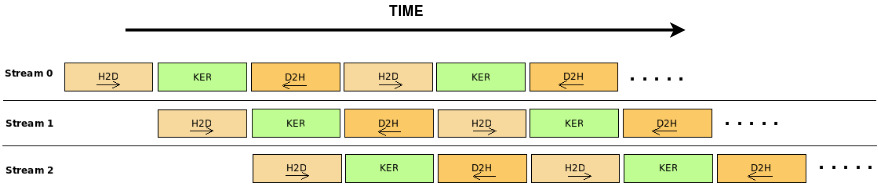
\includegraphics[width=\linewidth]{images/3Streams.jpg}
		\caption{Ideal behavior for 3 CUDA Streams.}
		\label{fig:threeStreams}
	\end{figure}

	To improve the potential for concurrent kernel execution, synchronization of any kind should be delayed as long as possible\cite{cudabestpractices}.
	So, we were careful to avoid \textit{Implicit synchronizations}\footnote{Implicit synchronization automatically happens when certain host operations are issued in-between commands given from different streams. E.g. this happens in case of: pinned memory allocations, device memory allocations, non-asynchronous memory operations etc.\cite{cudastrandconcurr}.} and all unnecessary \textit{Explicit synchronizations} \footnote{In CUDA there are several command to force synchronization either between host and device, or between streams.}.
	
	Another important face of overlapping, is that it requires to balance Kernels work in such a way it's sufficient to hide the time spent in data transfers, as we quoted just above. 
	This said we can have two possibly unfair scenarios:
	\begin{itemize}
		\item Data transfers take a small amount of time, while kernels are doing lot of computations;
		
		\item Data transfers take a big amount of time, with respect to time spent in kernel execution.
	\end{itemize}
	
	The former case may arise when we have a computation-intensive application or an \textit{irregular kernel}.
	By "irregular" we mean that we're facing an inefficient kernel, due to any flow control instruction (\texttt{if}, \texttt{switch}, \texttt{do}, \texttt{for}, \texttt{while}), that can significantly affect the instruction throughput by causing threads of the same warp to diverge, i.e. to follow different execution paths.\\ 
	If this happens, the different execution paths must be serialized, increasing the total number of instructions executed for this warp. When all the different execution paths have completed, the threads converge back to the same execution path\cite{cudaguide}.	
	So we should avoid different execution paths within the same warp.\\
	However, sometimes having short memory copy and long kernels can be profitable. As an example we'll see, in Chapter \ref{chap:experim}, that having more long kernels makes them to overlap more likely both in between them and with data transfers.
	% To obtain best performance in cases where the control flow depends on the thread ID, the controlling condition should be written so as to minimize the number of divergent warps. This is possible because the distribution of the warps across the block is deterministic
	% as mentioned in Section 4.1 of the CUDA C Programming Guide. A trivial example is when the controlling condition depends only on(threadIdx / WSIZE) where WSIZEis the warp size. In this case, no warp diverges because the controlling condition is perfectly aligned with the warps 
	
	
	The latter case in the above list, may happen when we move an amount of data such that it takes a huge amount time at each transfer, w.r.t. the amount it takes in calculations. So in this case the dominant overhead factor could be the data transfer.	
	%So about these two scenarios we had to make some assumptions and tunings, that we will see in ********. 

	
	\subsection{Occupancy of GPU cores}
	Once we carried out the stream logic, we had to understand how to try to exploit almost every Streaming Multiprocessor at any given time.
	This means that we wanted to launch as many kernels as needed to exploit SMs at their best, sometimes this means to arrive near the full \textit{\textbf{Occupancy}} of an SM for each kernel execution, in other situations it's better to decrease this resource exploitation\footnote{Chapter \ref{chap:experim} will also discuss occupancy and the role it played in our applications and experiments.}.
	
	Clearly, when we start an execution, we'll have a portion of time, a sort of \textit{"warm up" phase}, where we'll have first data transfers and kernels launches. So we'll have a narrowed number of running kernels. 
	But as soon as we could have enough data transfers, and therefore enough kernels to execute, we hope to reach a workload peak on GPU.\\
	In practice, when we just said \textit{lot of kernels}, we meant a lot of small groups of (data parallel) items on which (data parallel) computations have to be applied. So, each of these items will be assigned to one or more (few) thread blocks.\\ Now we'll better explain what Occupancy means.\\

	To \textit{\textbf{maximize utilization}} the application should be structured in such a way that it exposes as much parallelism as possible and efficiently maps this parallelism to the various components of the system to keep them busy most of the time\cite{cudaguide}.\\
	The main ways to maximize utilization can be classified as follows:
	\begin{enumerate}
			\item \textbf{Application Level}
			At a high level, the application should maximize parallel execution between the host, the	devices, and the bus connecting the host to the devices, by using \textit{asynchronous functions} calls and streams;
			
			
			\item \textbf{Device Level}
			At a lower level, the application should maximize parallel execution between the multiprocessors of a device.
			Multiple kernels can execute concurrently on a device, so maximum utilization can also be achieved by using streams to enable enough kernels to execute concurrently;
			
			
			\item \textbf{Multiprocessor Level}
			At an even lower level, the application should maximize parallel execution between the	various functional units within a multiprocessor.
			In particular, \textit{a GPU multiprocessor relies on thread-level parallelism to maximize utilization of its functional units}\cite{cudaguide}. 
	\end{enumerate}
	
	From the above, we can deduce that occupancy is directly linked to the number of resident warps\footnote{We recall that warps are groups of 32 threads running in parallel on a set of instructions. Resident warps are those warps that, at a given time, are active on a certain thread block. In Chapter \ref{chap:tools} we gave a detailed explanation of these concepts.}.\\
	At every instruction issue time, a warp scheduler selects a warp that is ready to execute its next instruction, if any, and issues the relative instructions to the active threads of the warp.
	The number of clock cycles it takes for a warp to be ready to execute its next instruction is called the \textit{\textbf{latency}, and full utilization is achieved when all warp schedulers always have some instruction to issue for some warp at every clock cycle during that latency period, or in other words, when latency is completely "hidden"}\cite{perfoptimize,understandlatency}. 
	
	The most common reason a warp is not ready, to execute its next instruction, is that the instruction's input operands are not available yet.\\
	If all input operands are registers, latency is caused by register dependencies, i.e. some of the input operands are written by some previous instruction(s) whose execution has not completed yet.\\ 
	So, in this case, the latency is equal to the execution time of the previous instruction and the warp schedulers must schedule instructions for different warps during that time\cite{cudaguide,understandlatency}.\\

	Another reason a warp is not ready to execute its next instruction, is that it is waiting at some \textit{memory fence} (\textit{Memory Fence Functions}) or synchronization point.\\ A synchronization point can force the multiprocessor to stay idle as more and more warps wait for other warps in the same block to complete execution of instructions.\\
	So, having multiple resident blocks per multiprocessor can help reduce idling in this case, as warps from different blocks do not need to wait for each other at synchronization points.
	
	The \textit{number of blocks and warps residing on each multiprocessor for a given kernel call depends on the execution configuration of the call} (grid and block dimensions), the memory resources of the multiprocessor, and the resource requirements of the kernel\cite{cudaguide}.\\
	Register and shared memory are others important Occupancy variables, but we didn't focused much on them as on execution configuration. This is because, in our applications, those factors had a negligible impact on eventual occupancy.\\
%	The number of registers used by a kernel can have a significant impact on the number	of resident warps. For example, for devices of compute capability 6.x, if a kernel uses 64 registers and each block has 512 threads and requires very little shared memory, then two blocks (i.e., 32 warps) can reside on the multiprocessor since they require 2x512x64 registers, which exactly matches the number of registers available on the multiprocessor. But as soon as the kernel uses one more register, only one block (i.e.,16 warps) can be resident since two blocks would require 2x512x65 registers, which are more registers than are available on the multiprocessor. Therefore, the compiler attempts to minimize register usage while keeping register spilling (see Device Memory Accesses)	and the number of instructions to a minimum. Register usage can be controlled using the maxrregcount compiler option or launch bounds as described in Launch Bounds.
%	Each double variable and each long long variable uses two registers.

At this point, we had to reason about how and when to maximize Occupancy in our Farm parallel pattern. We shouldn't forget that after looking for full occupancy, experiments can give a prove that a lower one could be better.\\
First, we have to make some assumptions:
\begin{itemize}
	\item no shared memory was used;
	\item we took a really poor amount of registers, given the really simple nature of our example Kernels \footnote{We'll see what kind of kernels we used to test the farm parallel pattern, with some code listings in \hyperref[chap:impl]{Chapter 4}.}.
\end{itemize}  
Anyway, our chosen kernels represent some \textit{important application categories}, as we mentioned in previous chapters.\\
Then we mainly put our attention on kernel \textit{execution configuration} and number of kernels launched (by different CUDA streams), in order to try to maximize the number of active warps inside each Streaming Multiprocessor.

\subsection{Occupancy drawbacks}
Occupancy is a very important factor to take into account, but it's more important to be aware that \textit{occupancy isn't the only factor to take care of}.\\
In other words, not always trying to achieve maximum occupancy is the best idea, in some cases lower occupancy gives even better performances.\\
It is common to recommend running more threads per Streaming Multiprocessor and/or running more threads per thread block; the motivation is that this is the main way to hide \textit{latencies}.\\
Indeed, common beliefs are: multithreading is the only way to hide latency on GPU; shared memory is as fast as registers\cite{cudaguide}. Those facts aren't always true.

Some studies demonstrated how was possible to hide arithmetic latency or to hide memory latency using fewer threads, leading to code that runs faster.
The \textit{Latency} is the time required to perform an operation, for arithmetic operations it takes \(\approx20\) cycles; for memory we have \(\approx400+\) cycles instead.\\
This, in particular, means that  we can't start a dependent operation during these times, but they can be hidden by overlapping with other (independent) operations\cite{loweroccupancy}.

\begin{lstlisting}
	x= a + b; // takes about 20 cycles to execute
	y = a + c; // independent, can start anytime(stall)
	z = x + d; // dependent, must wait for completion
\end{lstlisting}
So \textit{latency hiding} means to do other operations when waiting for latency, this will make code run faster (not faster than the peak). For example another way to hide latency is \textit{Instruction Level Parallelism}\footnote{In general ILP in a kernel is intended as assigning more instructions (possibly equal between them) to each single thread, instead of having a lot of threads executing a lower amount of instructions each. Furthermore ILP can be used to execute independent instructions between two dependent ones\cite{perfoptimize}.}.\\
Furthermore another common belief is that occupancy is a metric of utilization, but, as we anticipate, it's only one of the contributing factors\cite{loweroccupancy}.

Another type of latency is memory-bounded, let's take an example:
\begin{lstlisting}
	__global__ void memcpy( float *dst, float *src){
		int block = blockIdx.x+ blockIdx.y* gridDim.x;
		int index = threadIdx.x+ block * blockDim.x;
		float a0 = src[index];
		dst[index] = a0;
	}
\end{lstlisting}
To hide memory latency, using even fewer threads, we can do more parallel work per thread:
\begin{lstlisting}
	__global__ void memcpy( float*dst, float*src){
		int iblock= blockIdx.x+ blockIdx.y* gridDim.x;
		int index = threadIdx.x+ 2 * iblock* blockDim.x;
		float a0 = src[index]; 
		//no latency stall
		float a1 = src[index+blockDim.x]; 
		//stall
		dst[index] = a0;
		dst[index+blockDim.x] = a1;
	}
\end{lstlisting}
Note: threads don't stall on memory access, they stall on data dependency instead.

Performances improve copying more floats per thread, instead of copying one and run more blocks and allocate shared memory to control occupancy\cite{loweroccupancy}.\\
For example some common concepts\footnote{From CUDA Programming Guide.} on CUDA state that:
\begin{itemize}
\item "In general, more warps are required if the ratio of the number of instructions with no off-chip memory operands to the number of instructions with off-chip memory operands is low";  %()–No, we’ve seen 87% of memory peak with only 4 warps per SM in a memory intensive kernel. 
\item “For all threads of a warp, accessing the shared memory is as fast as accessing a register as long as there are no bank conflicts between the threads”\cite{cudaguide}. 
\end{itemize}
For the former there are studies that show how a reduced quantity of warps gives good performances on memory intensive kernels.\\
For the latter, in reality shared memory bandwidth is lower than register bandwidth, in fact we should use registers to run closer to the peak.
But requiring more registers can result in having a low occupancy.\\
So, in many cases, this can be accomplished by computing multiple outputs per thread (see above example on multiple floats copy)\cite{loweroccupancy,understandlatency}.

%P100: 10.6 TeraFLOPS of peak single-precision

\section{Overall Logic}
\label{sect:overallLogic}
We have an input stream of items, in particular they are small data parallel tasks, we don't know how much they are and their arrival frequency.
The logic of this work can be summarized in the following steps:
\begin{enumerate}
	\item In the beginning, as items arrive, we start to spread them among different CUDA streams, according to a Round-Robin policy;
	\item On a certain stream, say \texttt{streams[k]}, we send out a task (e.g. the \textit{k-th} item that has arrived from the input stream) to the device (GPU Global memory);
	\item Immediately after the data transfer call, we launch the kernel execution, with a certain \textit{execution configuration}\footnote{We recall that this is given by grid and block sizes that we set for a certain kernel call with the\\ \texttt{<<< grid, block >>>} syntax.}. The kernel call will be placed in \texttt{streams[k]} as well;
	\item Once the kernel ends its computations, we copy back to host, on \texttt{streams[k]}, the result data as output item;
	\item We'll send each result element onto the output stream. 
\end{enumerate}

	\begin{figure}
		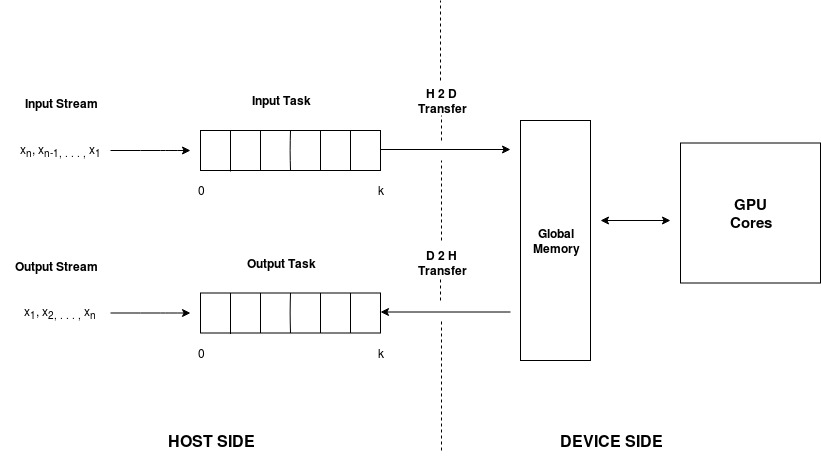
\includegraphics[width=\linewidth]{images/singleLogic.jpg}
		\caption{In this picture we show the schema of Farm on GPU, here we have only one task to/from the GPU.}
		\label{fig:H2D}
	\end{figure}
	
	This behavior is illustrated graphically in Figure \ref{fig:H2D}. Here we can see our input stream, from that at a given time we get a certain item, i.e. a task. In the diagram we simplified the concept of (data parallel) tasks, from the input stream, as it was a buffer of size \(k\); clearly this is only a graphical simplification. Then, we transfer the various items to Global memory of GPU.\\
	For reasons we showed in the previous sections, it would be unfeasible to work on single simple elements (e.g. float numbers) but, at the same time, we should maintain the pattern as close as possible to Stream parallel. That's why we're working on small data parallel tasks\footnote{We represented tasks as arrays, but they can be either small matrices or tiny images, as we'll see in \hyperref[chap:impl]{Chapter 4}.} of \(k\) items, where \(k\) is tested for several values but to remain a relatively small number of simple elements, possibly related to execution configuration on kernel, in particular to block size.\\

	Once we start to have several items available on GPU memory, they will be spread all over the SMs that will have enough available resources. Each task will be splitted in warps, so each active thread in a warp will compute one instruction per time, in parallel with other threads in the warp. The instruction that will be executed are essentially those specified inside kernel code.\\
	This means that we're executing in parallel the same operations over all the content in a task; in fact, as we mentioned before, each task is a small data parallel collection of items, upon which we're performing data parallel computations.  
	

	Since Figure \ref{fig:H2D} is a simplification, it may seems we're sending only one item per time to/from the GPU, this would correspond almost to a farm with one worker, processing one item per time. And this isn't completely what we wanted.\\
	\begin{figure}
		%	\hspace*{-2cm}  
		\vspace{-2cm}
		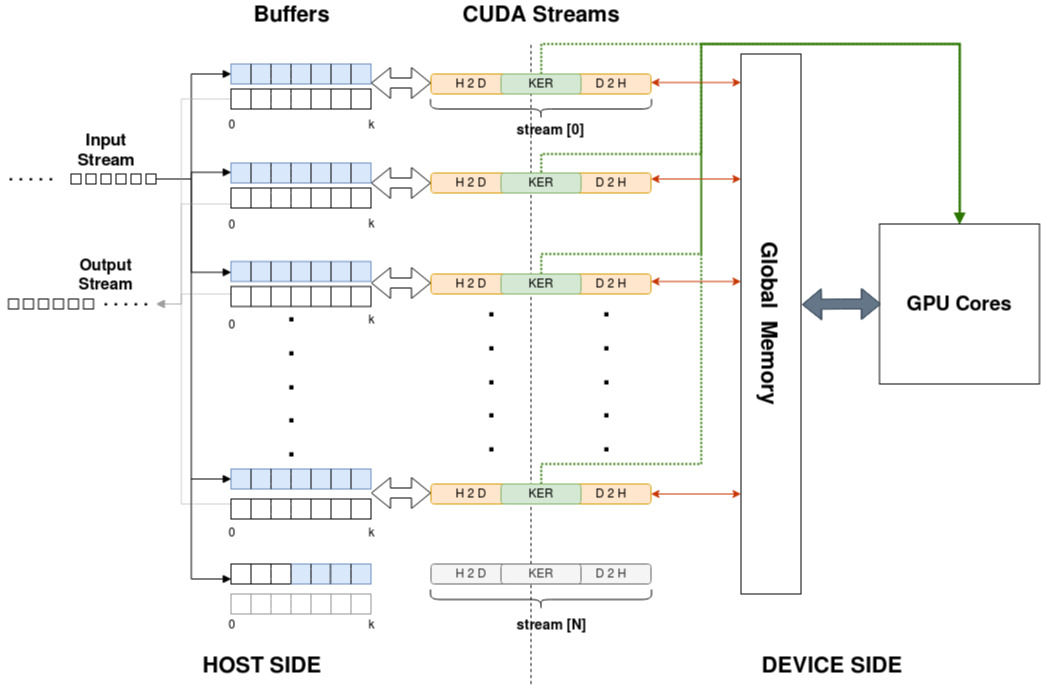
\includegraphics[scale=0.62,angle=-90]{images/overallLogic.jpg}
		\caption{Here we have an overall and broad graphical representation of our idea on how to fit a Farm parallel pattern on GPU architecture.}
		\label{fig:overallLogic}
	\end{figure}
	So, here's where CUDA Streams \footnote{Don't confuse input/output stream in Farm parallel pattern with CUDA Streams.\\ These are two completely different notions: the first is the parallel pattern input/output data type, the last are a CUDA feature (shown in \hyperref[subs:streams]{Section 2.3.3}).\\} are needed and we used them relying on the following ideas:
	\begin{enumerate}
		\item We have as many streams as Streaming Multiprocessors \footnote{Again CUDA Streams are a different concepts with respect to Streaming Multiprocessors. The first are a set of commands, the last are physical processing units inside the GPU.\\} and, at any given time, each of them hopefully issues a data transfer or a kernel executions;
		\item We should come to the point where each stream has issued at least one kernel launch, ideally we expect that each kernel execution is taken over by a certain multiprocessor. So, at a given time, we want to reach a work peak, where almost all SMs are busy;
		\item Obviously each kernel execution configuration should be well tuned, in order to take advantage of the maximum of resources in a multiprocessor (according to a certain kernel nature). 
	\end{enumerate}
	

	All of those parameters have been initially established taking into account of the NVIDIA GPUs' nature, then experimental proves have been performed\footnote{We'll see in next section more informations about Tunings.}. Measures and other estimation lead us to consider specific values for those variable parameters.\\
	So from the above facts is clear that we're exploiting each SM as a Farm parallel worker, furthermore, in such a way that all of those workers are as busy as possible. Note that our \(n_w\) \textbf{SMs-workers} apply a \textbf{kernel-function} \(f\) to all (data parallel) \textbf{tasks}.\\
	Bringing all pieces together we can summarize all project logic in Figure \ref{fig:overallLogic}.\\
	The schema may be further detailed as follows:
					
	\begin{itemize}
		\item We have \(N\) CUDA streams, where \(N\  (=n_w)\) is the number of Streaming Multiprocessors on the target machine;
		\item As input stream items arrive, in a Round-Robin way, we spread them all over the CUDA streams as follows:
		\begin{enumerate}
			\item As soon as we get the \(i^{th}\) task, it's asynchronously sent on \texttt{stream [i]} to the GPU, with the command \\ 
			\texttt{ \textbf{cudaMemcpyAsync}( devTask, hostTask, bytes, cudaMemcpyHostToDevice, \tab \tab \tab \tab stream [i]);}
			
			\item Immediately after we put kernel call, again on the \texttt{stream [i]}, to schedule the desired computations on that input item;
			
			\item Then, asynchronously again, we bring back results to host side, using the instruction \\
			\texttt{ cudaMemcpyAsync( devTask, hostTask, bytes, cudaMemcpyHostToDevice, \tab \tab \tab \tab stream[i]).}
			
		\end{enumerate}
	\end{itemize}

	
	Hopefully this approach should make each Streaming Multiprocessor (or at least a part) busy.
	Initially only few cores will be really busy, but as soon as CUDA streams get full, the pressure\footnote{In other words the amount of tasks assigned to each CUDA stream and so to each SM.} on the GPU should increase, so we expected that workload should be enough to almost fill all of Streaming Multiprocessors.\\
	\begin{wrapfigure}[20]{r}{0.4\textwidth}
		%\begin{center}
		%\raggedleft
		\centering
		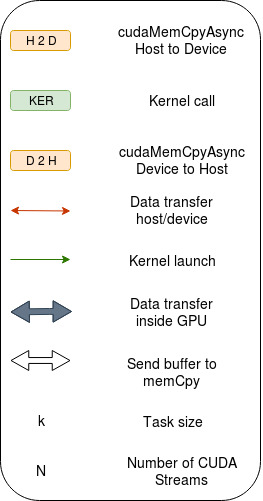
\includegraphics[width=1\linewidth]{images/logicLegenda.jpg}
		%\end{center}
		\caption{Legenda about Figure \ref{fig:overallLogic}.}
	\end{wrapfigure}
	In particular, for us this translates in trying to have, at any given time, the maximum number possible of active threads, having to execute instructions, inside each SM.\\
	Figure \ref{fig:singleStream} gives a closer look to what we just said.\\
	%Observing Figure \ref{fig:overallLogic}, w
	
	From that schema, looking at violet numbered labels, we can see the order in which we issue commands in a generic stream, and this will be the order in which commands will be issued to device side too, for that stream. \\
	The behavior of overlapping between different streams, isn't predictable\cite{cudaguide}. Anyway we should take advantage of the fact that, considering two different CUDA streams, we can overlap data transfer and/or kernel execution in a \texttt{stream [i]} with the ones in a \texttt{stream [j]} (for some \(j\in[0,N-1], \: for \: N =\# SMs\)). Obviously, when the number of CUDA streams is greater than 3, we can have only 2 data transfer operations executing at the same time (by two distinct streams)\footnote{As mentioned in \hyperref[chap:tools]{Chapter 2}, for concurrent memory copy between host and device, we have 2 copy engines.}.
	
	Note that in the Figure \ref{fig:singleStream} we represented a single kernel execution as fully occupying an entire SM; in reality not always we'll have this behavior, sometimes it's even convenient to not fully occupy an entire SM with a single kernel launch\footnote{We'll see how we practically tried out Streaming Multiprocessors \textit{occupancy} in  \hyperref[chap:experim]{Chapter 5}.}. \\
	
	Essentially if all of our reasoning and theories are right, we would expect that we can have an improvement, on completion time, roughly in the order of SMs number with respect to the \textit{serial approach}. \\
	This similarly means that if, for example, we have 3 CUDA Stream we would expect to take an advantage on approximatively 3 SMs (at peak work flow), so this should give us an improvement, in completion time, of at most 3 times compared to serial approach.\\
	The case of \textit{\textbf{serial approach}}, instead, processes input stream items without any type of overlapping, it is equivalent to:
	\begin{itemize}
		\item send an input task to device and wait on host for data transfer completion;
		\item call the kernel;
		\item host calls the copy back, from device to host, and keeps waiting until the end of data transfer;
		\item in the meanwhile kernel is running on GPU; 
		\item finally, only when all computations have ended up, results are transferred back to the host, that at this point finishes to wait for output and, so, it can continue with next task.
	\end{itemize} 
	

	\begin{figure}%[ht!]
			\hspace*{-0.5cm}  
		%\vspace{-2cm}
		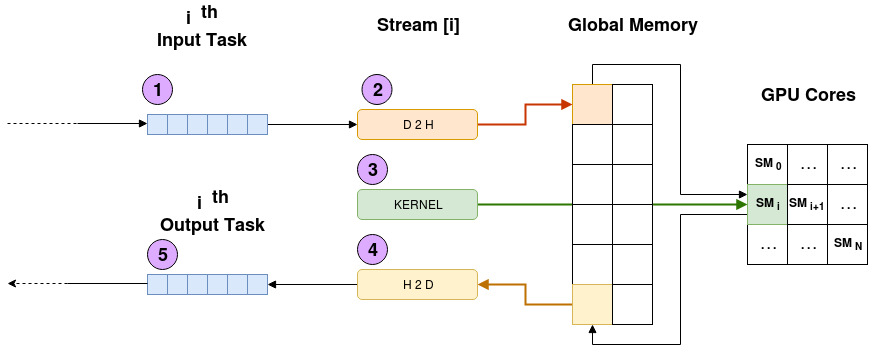
\includegraphics[scale=0.58]{images/singleTaskLogic.jpg}
		\caption{In this picture we can see what exactly happens in a certain CUDA Stream. Light violet numbered labels show the order in which commands are issued by host to the GPU by a generic stream.}
		\label{fig:singleStream}		
		
	\end{figure}	
\section{Tunings}
\label{sect:tunings}
	We showed a lot of peculiar behavior and architectural characteristics, as they were taken into account for different implementations, tests datasets and results analysis.\\
	It's clear that, once we decided how to organize our Farm parallel pattern for the GPU, we had to perform experiments and empirical evaluations.
	This is because:
	\begin{itemize}
		\item It was important to think about a general logic, that wasn't architecture-dependent\footnote{At least we can say that the overall view, showed in Fig. \ref{fig:overallLogic}, can be plausible with almost all NVIDIA's architecture having more than one copy engine and allowing concurrent kernel execution.};
		
		\item To validate our idea we had to make a lot of experiments, time measures, examples and counterexamples too;
		
		\item Clearly experiments required to get a little deeper about NVIDIA GPU's architecture, considering the good practices, apart from the considered application;
		
		\item Finally, we had to consider some feature totally application-bounded to launch tests and obtain results of interest.
	\end{itemize}
	
	So after the logical phase, we went through a \textit{tuning phase}, that first had to face general NVIDIA GPUs behavior and structure\footnote{In \hyperref[chap:experim]{Chapter 5} we'll mainly see tunings based on the GPUs used to run tests \textendash \textbf{P100} and \textbf{M40}.}.
	Some of the important best practices we introduced in tuning phase were:

	\begin{itemize}
		\item The effect of execution configuration on performance for a given kernel call generally
		depends on the kernel code, so experimentation is recommended\cite{cudabestpractices} and in fact we followed that approach;
		\item The number of threads per block should be chosen as a multiple of the warp size (generally equal to 32 threads) to avoid wasting computing resources with under-populated warps\footnote{For example, if we have a block size of 50 threads, the GPU will still issue commands to 64 threads, so we would waste 14 of them idling.}\cite{cudabestpractices};
		\item We exploited \textbf{\textit{Occupancy Calculator}}\footnote{Those tools are included in CUDA Toolkit, they provide mechanisms to choose thread block size based on kernel behavior, register and shared memory requirements.} both in spreadsheet and API functions\footnote{These are special functions to be called inside the code, we'll see in \hyperref[chap:impl]{Chapter 4} a code example on how and where they are used.} formats\cite{cudaguide}.
		 
	\end{itemize}

	Given those initial guidelines, it's important to highlight what are main variable parameters, in Figure \ref{fig:overallLogic}, on which the tuning was made:
	\begin{itemize}
		\item The number of CUDA streams;		
		\item The number of threads per block (block size);
		\item The number of blocks (grid size).
	\end{itemize}
	The first parameter changes mainly as the target machine changes\footnote{We'll see in Chapter \ref{chap:experim} that the experiments are performed on zero and three CUDA streams. Furthermore we test the case in which we have as many CUDA streams as SMs in the target GPU, so this value will change between P100 and M40 too.}.\\
	The second parameter, in our case, generally depends both on input tasks dimensions and CUDA limits on thread blocks dimensions. But the threads per block choice may be also influenced by the kernel nature and a tuning according to performance measures.\\
	The third is generally roughly determined dividing the size of the input data by the block size. However Farm is a particular case and sometimes may be useful to determine the grid size empirically.\\
	The \hyperref[chap:experim]{Chapter 5} shows all main parameters tested and their respective performances.
 
			 
\subsection{Tuning on block and grid dimensions}
	%It's important to understand some main concepts, that are the basis for the logic of this project.\\
	As we mentioned above, the variation on \textit{thread block size} and \textit{grid size}, can affect heavily performances, especially in an extreme scenario as the case studies of this thesis\footnote{Here we report some useful discussions on occupancy, block and grid dimensions from Stack Overflow:\\
		https://stackoverflow.com/questions/9985912/\\
		https://stackoverflow.com/questions/5643178/\\
		https://stackoverflow.com/questions/54715373/ }.
	There's a tight correlation in between \textit{Occupancy}, \textit{kernel execution configuration} and kernel code nature.
	First note that a certain block, whatever its dimension is, will be run on a single Streaming Multiprocessor and once it's assigned it will never be moved. When resources are allocated for a thread block in a SM, it will become an \textit{active block}.\\
	In a SM we can have multiple blocks running independently, each of which grabbing its portion of resources, i.e. we can have multiple active blocks on a SM until they don't hit the maximum allowed\cite{perfoptimize,cudaguide}.
	So, inside a certain SM, some particular cases may happen:
	\begin{enumerate}
		\item Maximum block dimension (meaning a lot of threads per block), can lead to have a smaller number of blocks\footnote{Even only one, as it happens for one of the applications we tested. Anyway, from best practices guide and from profiling this should be a inefficient configuration, so we should be very careful on performances from these situations.};
		\item Small block dimension, can give a higher number of blocks running on the same SM\footnote{We recall that GPUs have also a limit on the number of active blocks per SM.} .
	\end{enumerate}
	
	In the first scenario, we can have cases of good performances.
	For example, if few blocks have lot of work to do, it's more likely that they will monopolize resources of the SM in which they're active, making all other waiting blocks, scheduled in the same SM, idle for too long (for example in our GPUs it may happens for \textit{blocksize = 1024}). \\
	In the second scenario we can have cases of really poor performances due to low resources exploitation, but for some kinds of kernel we may have a gain, especially in cases as the above mentioned monopolization. So smaller blocks size, means more active blocks on a SM, at any given time. This may allow to have smaller and, so, faster blocks that allow new ones to start executing. Smaller block sizes eventually means to have more active blocks per SM\cite{cudabestpractices}.
	
	In general, there is a performance \textit{sweet spot} for middle values on thread block size (for example usually identified in \textit{blocksize = 512}).\\
	%To better explain that concept, let's take a simple example. It's the first type of kernel we tested \footnote{We'll take a closer look on that case study, with implementation details, in \hyperref[chap:impl]{Chapter 4}.}, so suppose we have:
	%\begin{itemize}
	%	\item Vectors of floats as input and output;
	%	\item We have a "regular" kernel, in other words inside that we have not irregular workflows, we haven't divergent execution flowsand workload between all threads is almost the same;
	%	\item We avoid all types of synchronizations, both thread synchronization (\texttt{\_\_syncthreads()}) and host/device one (\texttt{cudaDeviceSynchronize()}).
	%\end{itemize}
	%In this situation
	So our tests had to face the above explained behaviors too, without forgetting the nature of the various implemented kernels.


%\section{CPU/GPU Scheduling}
%\label{sect:cpugpuscheduling}
%In addition to the main logic of our project we introduced another branch of study.\\
%In particular, we extended the Farm parallel pattern on GPGPU introducing a sort of \textit{\textbf{CPU/GPU Scheduler}}.\\
%This consist in an implementation that, given an initial work percentage, it gradually and experimentally tunes those percentages to balance jobs.
%In particular, the scheduler adjusts the dimensions of data chunks directed to CPU or GPU on the basis of previous measured completion times of both devices.\\
%Clearly, starting from a user provided percentage, measured times are used to recompute percentages (and thus chunks dimension). So, in a finite number of algorithm steps, the two portion size will stabilize around two "good" values.\\
%This allow us to let host and device cooperate to apply same computations, but with different workloads. Clearly the main idea is to let GPU have a greater workload with respect to the one for CPU, so that  latter can be lighten from doing the entire computations; at the same time, having a good occupancy on GPU, we can gain a speedup compared to letting only one of the two processors doing all the work.\\
%
%	***************
%	qui dovresti dire che dipende dal tipo di computaz.
%	e in particolare dal rapport fra Tcomm e Tcalc ...
%************************



%******************
%LO SCHEMA GENERALE NON È SPIEGATO BENISSIMO.....
%******************